\documentclass[../../main]{subfiles}
\begin{document}

\begin{figure}[h]

\begin{center}
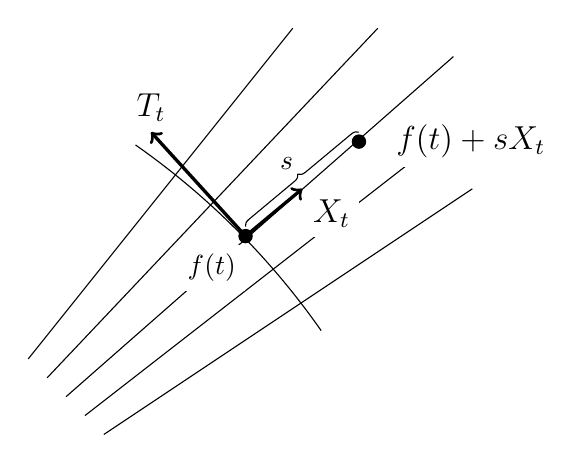
\begin{tikzpicture}[scale=1.2]
\draw (0,1.0) -- (2.8, 4.5);
\draw (0.2, 0.8) -- (3.7, 4.5);
\draw (0.4, 0.6) -- (4.5, 4.2);
\draw (0.6, 0.4) -- (4.2, 3.2);
\draw (0.8, 0.2) -- (4.7, 2.8);
\draw (3.1,1.3) arc (35:55:8cm);
\filldraw[black] (2.3,2.3) circle (2pt) node[anchor=north east, fill=white, yshift=-.1cm] {$f(t)$};
\draw[very thick, ->] (2.3,2.3) -- (1.3,3.4) node[anchor=south] {\large{$T_t$}};
\filldraw[black] (3.5,3.3) circle (2pt) node[right=10pt, fill=white] {\large{$f(t) + sX_t$}};
\draw[very thick, ->] (2.3,2.3) -- (2.9,2.8) node[anchor= north west, fill=white] {\large{$X_t$}};
\draw[decorate, decoration = brace] (2.3,2.4) --  (3.5,3.4) node[pos=.5, xshift=-.2cm, yshift=.2cm]{$s$};
\end{tikzpicture}
\caption{Ruled Surface}
\label{fig:ch02fig5}
\end{center}

\end{figure}
    

\end{document}